

\section{Y a-t-il eu au Moyen Âge un dialogue entre l’islam et le christianisme  - Remi Brague}
\sn{\cite{lejbowicz_y_2005}}

Je ne puis ici donner un panorama exhaustif d'une question si vaste et qui excède ma compétence. Je souhaiterais uniquement la poser de mon mieux. Il me faudra présenter le contexte d'ensemble, décrire l'espace et les orientations d'un dialogue éventuel, et souligner les contraintes qui l'ont empêché de se déployer.

\section{Le cadre historique}

\paragraph{Début de l'Islam inaccessible par le savoir}
Des débuts de l'islam, nous ne savons à peu près rien, ce qui s'appelle savoir. Les plus anciennes œuvres historiques écrites par des Musulmans ne furent composées qu'au IXe siècle, c'est-à-dire deux siècles après les événements qu'elles sont censées rapporter. Les témoignages proches ne sont pas moins orientés que les historiens musulmans, et ils sont de plus maigres et incomplets; ils nous donnent une tout autre image de "ce qui s'est vraiment passé". On a essayé d'écrire l'histoire de l'islam primitif en décidant d'ignorer systématiquement, par souci de méthode, tout ce que l'on ne peut pas dater. 
On a aussi réuni les témoignages des chroniqueurs, etc. non musulmans, de toute langue, pour les traduire en anglais et les soumettre à un examen critique.
Le plus ancien événement pour lequel on puisse indiquer une date certaine est la conquête arabe. Ce fait historique installe la scène sur laquelle la rencontre de l'islam et du christianisme a eu lieu. Notre plus ancien document est un papyrus, un reçu qui fut établi en 643 par un fonctionnaire arabe pour un paysan égyptien à qui l'on donnait quittance de l'impôt foncier versé aux conquérants. Cette guerre de conquête semble s'être déroulée comme toute autre guerre. Les Arabes n'ont été ni plus doux ni plus sanguinaires que les conquérants antérieurs, des Assyriens à Alexandre le Grand.

\paragraph{la conquête Islamique, rencontre entre Chrétiens et musulmans}
La conquête concerne le Moyen-Orient et l'Égypte, qui se trouvaient sous domination romaine - nous dirions «byzantine» -, la Perse\mn{il y avait aussi un important foyer chrétien en Perse cf \pageref{ChretienEnPerse}} qui avait sa dynastie nationale, les rives méridionales du bassin méditerranéen, et l'Espagne qui était dominée par les Wisigoths. Hormis la Perse, qui avait sa religion nationale, celle de Zoroastre, la majorité de la population - nous ne pouvons guère nous faire une idée précise de son nombre - était de religion chrétienne.
\paragraph{Une nécessaire cohabitation}Les conquérants arabes ne pouvaient ni massacrer ces gens ni les convertir en masse et d'un coup. Ils n'avaient d'ailleurs l'intention de faire aucune des deux choses. Cette cruauté aurait tué la poule aux œufs d'or. Selon une formule attribuée à 'Ali, les protégés sont «la matière des musulmans». De même, le Calife 'Umar aurait écrit à Abü 'Obeyda : \begin{quote}
    « Si nous prenions ceux qui y sont assujettis et que nous nous les partagions, que resterait-il aux musulmans qui viendront après nous ? Ils ne trouveraient, pardieu, plus personne à qui parler ni du travail de qui profiter !»
\end{quote} 

\paragraph{une asymétrie entre monde chrétien et monde musulman}
C'est ainsi que naquit une situation qui contribua de façon essentielle à déterminer la possibilité et le déroulement d'un dialogue entre religions. Elle est caractérisée par une asymétrie. Il y a dans l'espace musulman des chrétiens. Ils possèdent dans la cité islamique une place définie par le droit. En revanche, il n'y a en
terre de chrétienté, en théorie du moins, que des chrétiens et des juifs. Pour le monde islamique, les chrétiens sont donc aussi bien
<<dedans» que «dehors». Pour le monde chrétien, à l'opposé, les musulmans ne sont que «dehors». Ce n'est que de façon exceptionnelle et provisoire que des musulmans vivent en terre chrétienne.

\paragraph{quelques exceptions de musulmans en monde chrétien, mais pas d'élite}
Cela se produit là où des armées chrétiennes occupent des régions qui étaient sous domination musulmane. Ceci ne concerne guère, cependant, que les musulmans de base, paysans ou artisans ; les «intellectuels» ne restaient généralement pas sous domination chrétienne : liés au pouvoir, ils partaient avec lui. On a quelques exemples de ce genre de situation. La frontière entre l'Islam et l'Empire romain d'Orient n'est pas stable. Dans la guerre entre celui-ci et les califes, la ligne de front se déplace en Syrie, parfois assez vite. Au xe siècle, les Byzantins ont à nouveau le vent en poupe. Des villes comme Alep passent tour à tour sous domination chrétienne et musulmane. En Europe, on peut citer certaines régions d'Espagne, après la conquête, ce qu'on appelle la \textit{reconquista} du sud islamique par les royaumes chrétiens du Nord. C'est le cas de Tolède sous le règne d'Alphonse le Sage. Même cas de figure en Sicile à partir de la seconde moitié du XIe siècle, moment où les Normands prennent d'abord Messine (1061) et un peu plus tard Palerme (1072).
\paragraph{faible impact des croisades dans le monde musulman}
Les Croisades, à partir de 1096, n'ont éveillé dans le monde musulman qu'un écho faible et tardif \mn{voir Tolan}. Ainsi, le plus grand intellectuel de l'islam médiéval, et peut-être de l'islam tout court, al-Ghazalï (m. 1111), qui vivait pourtant dans la région, n'y fait nulle part allusion et semble ne pas les avoir remarquées. Ce n'est que bien plus tard, pas avant le XIXe siècle, qu'elles furent montées en épingle comme symbole de la rencontre manquée entre Orient et Occident.

%---------------------------------------------
\section{Le contexte social}

\paragraph{pas de liberté de penser}
À l'intérieur des deux domaines, le contexte des rencontres entre religions est lui aussi asymétrique. Dans chacun d'eux, une religion déterminée est la religion dominante, celle que )'on pourrait appeler, non sans anachronisme, la religion de «l'Etat». Les
gouvernants se réclament de cette religion comme à un des principes de leur légitimation. Il ne peut donc être question de permettre ce que nous appelons la «liberté de penser». En chercher l'équivalent au Moyen Âge serait parfaitement anachronique.

\paragraph{une exception : la conquête de Bagdad par les Mongols}
La seule exception, celle qui confirme la règle, le seul cas de neutralité de la puissance politique vis-à-vis des religions, est présentée par la situation qui s'était créée dans une partie du monde musulman, entre 1258 et 1290. La première date est celle de la prise de Bagdad par les Mongols. Les vainqueurs étaient bigarrés en matière de religion : il y avait parmi eux des musulmans, mais aussi des chrétiens d'obédience nestorienne, des bouddhistes, des chamanistes. Les khans n'avaient pas de religion déterminée à imposer aux vaincus, et n'en imposèrent donc aucune non plus. Une telle atmosphère permit notamment l'œuvre d'Ibn Kammü.na, qui mena entre les trois religions une comparaison qui, pour l'époque, faisait preuve d'une grande objectivité\mn{Ibn Kammuna a passé quasiment toute sa vie à Bagdad. Il y a vécu le renversement du pouvoir musulman par les troupes Mongoles de Houlagou Khan en 1258. À la suite de cela, les Mongols ont établi pour une trentaine d'années leur politique traditionnelle de tolérance religieuse, amenant avec eux une population qui comprenait chamanes, nestoriens, bouddhistes, musulmans etc. Les musulmans sont restés majoritaires dans les territoires conquis, mais cette société  n'était plus réglementée par les principes de l'islam. Il a porté un regard parfois très critique sur l'islam, mais il a aussi témoigné d'une forme d'estime pour cette religion ainsi que pour le christianisme, notamment par ses éloges de Mahomet et de Jésus. Ses écrits attestent de son attachement au judaïsme.}. Cela dura jusqu'en 1290, lorsque le Grand Khan de l'époque décida d'adopter la religion qui était déjà devenue celle de la majorité de ses nouveaux sujets, c'est-à-dire l'islam.
\paragraph{la dhimma}
Le système islamique de la \textit{dhimma}  consiste à tolérer des communautés non musulmanes, pourvu qu'elles possèdent un livre saint. Les «païens», en revanche, n'ont en principe que le choix entre la conversion ou la mort. Juifs et chrétiens sont soumis à diverses mesures explicitement destinées à leur faire comprendre, en les humiliant, l'intérêt qu'ils auraient à adopter l'islam. C'est ainsi qu'ils doivent payer un impôt spécial, se vêtir de couleurs spécifiques, renoncer à certaines montures, ne pas construire de nouvelles églises, éviter de faire sonner leurs cloches ou de chanter l'hymne trop fort, etc. Quant à ses conséquences sociales, ce système fonctionne un peu comme une nasse où l'entrée est libre et la sortie interdite. On est en droit d'adopter la religion des souverains, voire, on y est encouragé. Il est en revanche strictement défendu, en principe sous peine de mort, de la quitter en faveur d'une autre. Le christianisme médiéval appliquait d'ailleurs des règles analogues
aux Juifs, les unes dès avant l'islam, certaines inspirées de lui, comme la rouelle de couleur jaune.

\paragraph{conversion collective comme norme}
Au Moyen Age, sauf rares exceptions, la conversion vient d'en haut. Les chefs prennent des décisions en matière de religion, c'està-dire aussi en matière de politique; le peuple suit en bloc la classe dirigeante. C'est de cette façon que les tribus dites <<barbares» se laissaient baptiser comme un seul homme, une fois que leur chef s'était déclaré prêt à adopter le christianisme. Cela se passa ainsi pour Clovis, et plus tard dans l'Est et le Nord de l'Europe, jusqu'au dernier peuple à accepter le baptême, aussi tard qu'en 1386, les Lituaniens.


Des phénomènes analogues se produisirent quand par exemple l'Indonésie adopta l'islam: le rajah local se faisait musulman, son peuple suivait en masse. La conscience d'une valeur indépendante de l'individu était à l'époque plutôt une exception qu'une règle. On a un exemple d'une telle exception dans un récit sur la conquête arabe : un général musulman, passant en revue une tribu victorieuse, constata qu'elle était chrétienne. Il exigea qu'elle passât à l'islam, qui devait être l'unique religion des Arabes. Tous acceptèrent, sauf un certain Layth, qui subit le martyre. Sans cet acte de courage, nous ignorerions tout des faits.


\section{Le contexte intellectuel}

\paragraph{une langue commune, l'arabe ou des langues par communauté}
Entre la situation de la chrétienté et celle du monde islamique, on observe une différence capitale. Dans le premier cas, chaque communauté religieuse possède sa langue de culture, qui est selon les régions le grec ou le latin. Dans le second, même si les communautés chrétiennes gardent longtemps une langue liturgique bien à elles, comme le copte ou le syriaque, il se met en place assez rapidement une langue de culture commune, qui est l'arabe. Celui-ci est langue de l'administration depuis 750. Quant à la possibilité d'un dialogue entre religions, le fait entraîne des conséquences positives et négatives. Dans le monde islamique, la présence d'une langue commune permet, c'est l'aspect positif, une intercommunication très facile. En revanche, les non-musulmans peuvent être compris sans trop de difficulté de leurs souverains musulmans et doivent donc prendre leurs précautions. 1.;usage d'un alphabet différent ne suffit que jusqu'à un certain point. Une attaque frontale contre la religion dominante est à peu près impensable.
On voit bien les conséquences quand on compare la situation des Juifs en chrétienté et en terre d'islam. En terre chrétienne, les Juifs emploient, dans la vie quotidienne, la même langue que les chrétiens, à savoir le vernaculaire local. Mais si l'on se place au niveau du savoir religieux et, socialement, dans le milieu des clercs de chaque religion, les conditions du dialogue intérieur avec le judaïsme deviennent analogues à celles qui déterminent le dialogue extérieur entre Islam et Chrétienté. Les rabbins et les clercs chrétiens n'écrivent pas la même langue, mais, respectivement, l'hébreu et le latin ou le grec. Les oulémas écrivent l'arabe, alors que leurs adversaires chrétiens s'expriment en grec ou en latin. D'où un dialogue de sourds. Par ailleurs, écrire sa propre langue offre une protection qui permet aux hétérodoxes de dire ce qu'ils ont sur le cœur. Les Juifs peuvent par exemple mettre en circulation les Toledot Yeshu, qui offrent une version anti-chrétienne de l'histoire du Christ. Les choses ne s'envenimèrent que lorsque des transfuges mirent en garde leurs nouveaux coreligionnaires contre le contenu des livres de la religion de leurs pères.

\paragraph{bonne connaissance de l'Islam par Byzance}
À l'intérieur même de la chrétienté, il y a des différences entre
l'Orient et l'Occident. Byzance connaît l'islam relativement bien, et relativement tôt, avant même que la dogmatique islamique ne se cristallise. Ainsi, la polémique de saint Jean Damascène, peu avant le milieu du vrne siècle, nous présente un état des questions disputées dans l'islam de l'époque7. Le Coran est traduit en grec dès le 1xe siècle, d'ailleurs pour pouvoir être réfuté plus efficacement.

En revanche, les européens connaissent l'islam assez mal. Pour eux, les musulmans sont simplement des païens. Cette façon de voir a aussi des raisons concrètes. Le premier contact avec des musulmans ouvrit en effet un second front au sud, alors que l'Europe était
déjà assiégée au nord par les Normands. Comme l'Europe croyait elle-même représenter la chrétienté, elle considéra ses ennemis comme étant, globalement, des païens. Dans une situation d'urgence, des nuances plus subtiles n'avaient guère leur place. D'où la caricature que l'on trouve encore dans la \textit{Chanson de Roland}: le «sarrasin» est un idolâtre, qui adore trois divinités, parmi lesquelles :figure aussi Muhammad.

\paragraph{XIIè : Pierre le Vénérable}
Ce n'est qu'à partir du xiie siècle que le portrait-charge naïf le céda à une vision plus nuancée de l'adversaire. Pierre le Vénérable, abbé de Cluny (m. 1156) fit traduire en latin le Coran ainsi que d'autres œuvres donnant une idée plus juste et plus précise de l'iJlam. Ce dossier produit par des érudits réunis dans la vallée de l'Ebre forme ce que l'on appelle la \textit{collectio toletana}. Mais le manuscrit qui le contient n'a à peu près pas circulé, et son contenu ne fut imprimé qu'au XVIe siècle.
\paragraph{XIII : Roger Bacon  et Lulle}
Au xiiie siècle, le besoin se fit sentir d'une meilleure connaissance de l'islam. Le franciscain Roger Bacon (m. 1292) fit figurer parmi l'ambitieux programme de réformes qu'il soumit au pape la fondation d'écoles de langues qui devraient enseigner entre autres l'arabe. Raymond Martin, un dominicain catalan, se familiarisa suffisamment avec l'arabe et l'hébreu pour pouvoir écrire son célèbre \textit{Pugio fidei adversus mauros et judaeos} (1278), dont le titre indique bien l'intention polémique. Raymond Lulle (1233-1315), catalan originaire de Majorque qui avait été reconquise peu avant sa naissance, se donna la peine d'apprendre l'arabe pour composer en cette langue des présentations du christianisme à l'usage des arabophones, lesquelles semblent malheureusement avoir été toutes perdues.



\section{Le contexte affectif}

La connaissance de chacune des deux religions par l'autre est souvent assez mauvaise. Mais ce n'est pas pour les mêmes raisons. Il importe de se rendre compte des obstacles. Ils sont symétriques, mais inversés. Pour le dire en une formule évidemment sommaire : \textbf{les chrétiens savent qu'ils ne connaissent pas l'islam; les musulmans croient qu'ils connaissent le christianisme.}

\paragraph{Difficulté à penser l'Islam pour le Christianisme}
Pour le christianisme, l'islam est quelque chose qui n'aurait pas dû exister. L'islam est un imprévu, quelque chose de nouveau et d'inattendu, et donc de paradoxal. Les Chrétiens en tant que tels savent, ou croient savoir, ce que c'est que le judaïsme et ce que c'est que le paganisme. Or, les musulmans ne se laissent pas classer dans une catégorie préexistante: l'islam n'est pas païen- en tout cas il est monothéiste ; il n'est pas non plus juif; il est encore moins chrétien. C'est ce qui expïque une surprise qu'on n'a pas de mal à sentir chez les Pères de l'Eglise qui ont eu à faire avec l'islam. Ainsi Jean Damascène, déjà cité, considère l'islam comme une hérésie chrétienne.

\paragraph{Le Christianisme est réduit/ordonné dans l'Islam}
Rien de tel pour l'islam. Pour lui, le christianisme est quelque chose de bien connu, une vieille histoire. Le Coran contient des renseignements sur les chrétiens : ils adorent à côté du Dieu unique d'autres entités, comme Jésus et sa mère. Le christianisme est quelque chose de dépassé. Les chrétiens se sont refusés à reconnaître le prophète définitif qui devait parachever leur religion. Ils ont manqué le coche. De plus, ceux des chrétiens concrets qui sont présents sous domination musulmane, divisés en sectes qui s'anathématisent réciproquement, et maintenus dans une humiliation commune, ne semblent pas avoir grand-chose d'intéressant à enseigner.

\paragraph{Asymétrie psychologique}
De telles façons de voir ont des conséquences quant aux affects fondamentaux de chaque religion envers les autres. Nous n'éprouvons pas face à l'inconnu les mêmes affects qu'envers ce qui nous est familier. Quand les choses se passent bien entre les deux religions, l'islam est aux yeux des chrétiens un objet de curiosité qui peut fasciner, une sorte d'\textit{enfant terrible} que l'on regarde avec une tendresse indulgente ; quand au contraire les choses vont mal, il devient un objet de haine et de crainte.

\paragraph{pas de curiosité de l'Islam pour le Christianisme}
Réciproquement, quand les choses vont bien, le christianisme est pour l'islam un objet de sympathie, cette sympathie condescendante que l'on a envers un vieil oncle un peu gâteux et qui rabâche toujours les mêmes histoires. Mais il n'est en aucun cas un objet de curiosité. La curiosité envers l'autre est d'ailleurs une attitude typiquement européenne, rare hors d'Europe, et exceptionnelle en Islam. Quand les choses vont mal, l'islam éprouve envers le christianisme beaucoup moins de la haine que du mépris.


En dernière instance, cette attitude dépend directement de la place que les deux religions occupent dans l'histoire. Très platement: l'une vient avant l'autre. Mais cet ordre n'est pas que chronologique. Il a été l'objet d'une réflexion. Très tôt, à vrai dire dès qu'il s'est constitué comme une dogmatique indépendante, l'islam s'est compris comme un post-christianisme: les plus anciens textes de style coranique que l'on puisse dater sont les inscriptions du Dôme du Rocher, à Jérusalem, qui attaquent la Trinité. L'islam se voit comme la dernière religion, la religion définitive, celle qui relève le judaïsme comme le christianisme, au sens de la « relève » telle que le concevait Hegel (\textit{Aufhebung}), laquelle tout à la fois abolit et assume ce qui la précède et la prépare.

\section{Esquisse de la littérature apologétique}

Je ne puis ici risquer qu'un coup d'œil rapide et pour l'essentiel de seconde main sur la littérature polémique et apologétique
\paragraph{littérature apologétique : constitutive de l'Islam}
Elle s'adresse avant tout à ceux qui partagent la religion de leur auteur. Elle est à usage interne. Il ne s'agit pas de convaincre l'autre de se convertir en montrant les beautés de sa propre religion. Il s'agit bien plutôt de décourager ses coreligionnaires d'abandonner leur foi en faveur d'une autre religion, dont on devra donc faire ressortir les absurdités. Cela n'encourage guère l'objectivité, encore moins l'effort pour comprendre avec sympathie la position de l'autre.
La situation n'est pas la même pour le christianisme et pour l'islam. Le christianisme a dû se séparer du judaïsme, du paganisme,
de la gnose, de ses propres hérésies; en revanche, il n'a bien évidemment pas eu à se définir en se distinguant de l'islam qui n'existait pas encore. Alors que celui-ci entre en scène, la dogmatique chrétienne est en place depuis des siècles. En revanche, l'islam a dû se définir contre un christianisme qui était déjà là. La polémique contre le christianisme (et déjà contre le judaïsme) n'est pas pour l'islam secondaire, elle est constitutive. Le premier livre de polémique anti-chrétienne de l'islam n'est autre que son tout premier livre en général, c'est le Coran.

\paragraph{Risque du synchrétisme chez les musulmans}
Plus tard, la polémique fut rendue nécessaire non pas malgré les conversions à l'islam, mais, paradoxalement, par le mouvement même de ces conversions. Se faire musulman est très facile. Il suffit de prononcer devant témoins une courte formule de confession de foi (\textit{shahiida}). Le catéchisme auquel on adhère est bref et assez plausible \mn{Eglise vs Secte}. Et les musulmans n'ont pas l'habitude de mettre à l'épreuve la conviction du néophyte. Une telle attitude ne manque pas d'avantages évidents. Mais elle fomente un danger, celui du syncrétisme chez des gens qui ne se sont convertis que pour la forme ou sans vraiment savoir à quoi ils s'engageaient, et qui cherchent à introduire dans l'islam le plus possible du contenu de leur religion précédente. L'islam craint donc de se dissoudre dans une vague religiosité composite. La polémique sert à immuniser les musulmans contre le christianisme.
\paragraph{contre les affirmations christologiques, la Trinité, la falsification de la Bible}
Les contenus de cette polémique sont toujours les mêmes et roulent sur les grands thèmes de la christologie et de la Trinité, de la Bible: a-t-elle été corrompue par ses porteurs ou gardée intacte? Muhammad y a-t-il été prédit? De temps en temps, elle prend une allure sociale, et les musulmans se plaignent de la trop grande influence des chrétiens, médecins par exemple, dans la société. Le thème d'une corruption historique du christianisme mise au débit de saint Paul n'apparaît qu'au xme siècle avec 'Abd al-Jabbar, qui a peut-être utilisé des textes judéo-chrétiens.

\paragraph{Une religion par la force, quel signe du Prophète}
Les arguments sont eux aussi récurrents. Ainsi ceux des chrétiens: comment une religion est-elle venue au pouvoir, pacifi-
quement, ou par la force des armes? À quoi reconnaît-on l'authenticité de la mission d'un prophète ? Est-elle corroborée par des miracles? Le prophète se distingue-t-il par un mode de vie particulièrement édifiant? Ces questions d'allure purement historique sont biaisées: il s'agit de faire ressortir le caractère militaire de l'expansion de l'islam, l'absence de miracles chez Muhammad, sa vie sexuelle agitée. Dans ce genre de littérature, tous les arguments sont bons, pourvu qu'ils frappent l'adversaire. On comprend que la lecture de ces textes ne donne pas une idée très positive de la nature humaine...

\section{Dialogues ?}

\paragraph{Caractère fictif des vrais dialogues}
En fait de dialogues, nous possédons avant tout des œuvres littéraires qui se présentent comme si elles reproduisaient des discussions réelles entre les représentants de diverses religions. Mais il s'agit de fictions. C'est le cas du \textit{Dialogue entre un philosophe, un juif et un chrétien} de Pierre Abélard (vers 1140), dans lequel le philosophe est un musulman, peu orthodoxe il est vrai. C'est aussi le cas du \textit{De pace fidei} écrit par le cardinal Nicolas de Cuse au lendemain de la prise de Constantinople (1453), ou encore du \textit{Colloquium Heptaplomeres} que le juriste français Jean Bodin écrivit probablement vers 1593.
De véritables dialogues entre des personnages réels où chacun exprimerait dans son vocabulaire à lui ses convictions authentiques, restent une exception. On cite partout une disputation de ce genre, censée avoir eu lieu à Bagdad. Les représentants de chaque opinion, même les moins admises, y auraient pu s'exprimer librement, tous se seraient mis d'accord pour s'abstenir d'argumenter sur la base d'un texte scripturaire, etc.14 Il n'en faut pas moins pour enflammer l'imagination« multiculti » de nos belles âmes. L'anecdote provient en fait d'un orthodoxe des plus étroits, qui ne la rapporte que pour
dire son scandale \sn{Abu 'Umar ibn Sa'dï, dans le dictionnaire biographique de al-Jumaydi, Le Caire,
19 5 3 ; encore cité récemment dans L. E. GoonMAN, Jewish and Islamic Philosophy. Crosspollinations
in the Classic Age, Edimbourg, 1999, p. VII.}. N'aurait-il pas, sinon tout inventé, du moins considérablement forcé le trait?

\paragraph{Caractère polémique et institutionnel des dialogues}
La plupart du temps, le contexte des dialogues est polémique. On peut signaler la \textit{disputatio} tenue le 30 mai 1254 à Karakorum, en présence du khan des Mongols Mongke, à laquelle prirent part le franciscain flamand Guillaume de Ruysbroek (Rubruquis), envoyé de Louis IX et du pape, des chrétiens nestoriens, des bouddhistes et des musulmans. Mais notre seule source est le franciscain lui-même, qui s'est sans doute, et bien naturellement, donné le beau rôle.
Entre juifs et chrétiens, les disputations (\textit{wikkuah}) sont institutionnalisées. Les juifs sont contraints à disputer, la plupart du temps pour répondre aux accusations d'un de leurs coreligionnaires passé au christianisme. Cela ne se fait pas sans une certaine équité. Ainsi, le roi d'Aragon, pourtant chrétien, déclara vainqueur le rabbin de Gérone Nahmanide dans la polémique qui, à Barcelone, en 1263, l'opposait au converti Pablo Cristiani, et lui décerna même une récompense en argent. Reste que l'atmosphère de tels débats est dans l'ensemble désagréable, la pression sociale s'exerçant en sens unique. Elle ira d'ailleurs en s'accentuant jusqu'à l'expulsion finale de 1492.

\paragraph{Quelques exceptions}
Entre chrétiens et musulmans, les disputes publiques n'ont pas
de caractère institutionnel et sont plus rares. Les légendes ne manquent pas, par exemple à propos de saint François. Raymond Lulle
:fit une tentative de ce genre à Bougie, et y fut lapidé. On a peut-être un cas, mais notre seule source à ce sujet est un poème espagnol,\textit{ La Disputa que fue ficha en la çibdad de Feç delante del Rey e de sus sabios}, supposé écrit à Nicosie (Chypre) en 1469, et rapportant une dispute tenue à Fez en 139417. Elle se serait terminée par la conversion du principal docteur de la Loi musulmane (\textit{faqïh}) de Fez. On peut y voir, pour dire le moins, une certaine stylisation ... Il est en tout cas
intéressant que la dispute se serait déroulée à propos d'un livre sur la Trinité et l'Incarnation, écrit en arabe, intitulé \textit{Condus} (peut-être \textit{Quddüs}, « très saint»), et œuvre de Raymond Lulle. Par ailleurs, le climat global de tolérance semble correspondre assez bien à la réalité de l'époque.


\section{Conclusion: « prêcher des convertis »}

Ainsi, au Moyen Âge, les véritables dialogues entre islam et christianisme sont des plus rares, et, si l'on entend par-là des dialogues tels que ceux qui nous semblent souhaitables, simplement inexistants. La littérature polémique s'adresse à des gens déjà convaincus. Le dialogue est plutôt un genre littéraire qu'une réalité. Les essais de traiter l'autre avec équité, et, déjà, de bien le comprendre, restent une exception. On a certes de droit de rêver à de tels dialogues entre religions pour l'avenir. Mais rien ne nous autorise à projeter ce rêve dans le passé médiéval. Notre entreprise est peutêtre noble, mais elle ne doit pas sa noblesse à de quelconques ancêtres.


\section{Discussion}
 M. Alain BESANÇON. - J'ai relevé des points qui peuvent introduire des discussions plus vastes. La conquête, par le bas, de façon pacifique, de la société par les chrétiens ne va durer que jusqu'à Constantin. Ensuite la conversion s'est souvent opérée par le sommet. Celle de l'Allemagne, du Nord en particulier, s'est faite par le fer et par le feu - d'une façon assez musulmane - et la conversion de la Scandinavie, de la Pologne, de la Russie, de la Hongrie, dans toute l'Europe de l'Est et du Nord s'est faite par les princes. Ce sont les princes qui baptisaient leurs sujets, les plongeaient dans les rivières et les lacs pour recevoir le sacrement. Au sujet des conquêtes de l'Islam, il faut se souvenir que les Arabes n'étaient pas tellement nombreux. J'ai l'impression qu'il y a eu un mouvement de boule de neige. En un siècle, ils sont allés des frontières de la Chine à Poitiers. Cela a été permis par une conversion simultanée de masses chrétiennes à l'islam et, en particulier, de toutes les églises travaillées par l'hérésie (nestoriens, monophysites, donatistes, ariens d'Espagne). Pour l'Espagne, il est je crois reconnu que la conquête de l'Islam par les Arabes est facilitée par un retour de flamme de l'arianisme. Les chrétiens sont devenus rapidement musulmans. Ils ont ouvert les portes aux petites troupes conquérantes. Les juifs, que l'on tracassait depuis des siècles, ont aussi ouvert les portes aux conquérants musulmans en espérant qu'ils les laisseraient davantage en paix.
Vous avez dit que toutes les œuvres de Raymond Lulle ont disparu. Il existe pourtant son Livre du gentil est des trois sages où il imagine un dialogue entre les trois religions.
\newline M. Rémi BRAGUE. - Ce sont les œuvres arabes qui ont disparu. Sinon, il reste beaucoup d'œuvres de Raymond Lulle, qui est un auteur extraordinairement prolifique.
\newline M. BESANÇON. - Il me semble qu'il n'a rien compris à l'islam. Il n'a fait que projeter son christianisme sur l'islam.
La protection de la dhimma a touché les juifs, les chrétiens, les zoroastriens et ce que l'on a appelé les sabéens. Elle n'a pas touché les hindouistes. C'est pour cette raison que la conquête de l'Inde par l'Islam a été d'une telle cruauté: les hindouistes étaient considérés comme des kafirs, des infidèles. Ils avaient donc le choix entre la conversion à l'islam, qui s'est souvent produite, et la mort ou l'esclavage.
Vous avez touché à une équivoque dont nous allons parler certainement dans la journée: les musulmans sont-ils des païens ou non?
Intervenant non identifié. - Doit-on écrire Islam avec une minuscule ou avec une majuscule ?
\newline M. BRAGUE. -  C'est une convention adoptée par certains savants occidentaux, et français évidemment puisque nous avons la chance d'avoir une langue où il y a des majuscules et des minuscules. C'est un moyen commode de trouver pour l'Islam l'équivalent de cette distinction qui existe dans les langues européennes entre christianisme - la religion - et chrétienté, Christendom et Christianit:y, Christantum et Christenheit. C'est facile dans les langues de l'Europe. En français, il n'y a qu'un mot.
L'islam, avec une minuscule, est le nom commun qui désigne l'attitude d'abandon de soi sans réserve dans les mains de Dieu: il s'agit de la religion musulmane. L'Islam, avec une majuscule, est un nom propre qui désigne une réalité historique et géographique: il s'agit du monde musulman, de la civilisation musulmane.
Lorsque j'ai esquissé cette symétrie entre christianisme et islam primitif, je voulais expliquer une seule chose, à savoir la constitution d'une chrétienté - l'Empire romain - et la constitution de l'Islam - l'Empire arabe. Pour la suite des opérations, effectivement, il y a aussi une symétrie. Le christianisme, devenu chrétienté, s'est étendu par des moyens aussi bien militaires que pacifiques. Des missionnaires étaient en même temps des soldats, parfois dans la même personne, comme les chevaliers Teutoniques et les chevaliers PorteGlaive. En Islam, réciproquement, il y a eu aussi bien une poursuite de l'expansion militaire - vous avez fait allusion à ce sympathique personnage, Mahmüd de Ghazni, que l'on n'a toujours pas oublié aux Indes-, mais il y a eu aussi une expansion pacifique qui se faisait, de la même façon, par conversion des princes. Ainsi, à une époque plus proche de nous, l'Indonésie est devenue musulmane. Les radjahs se sont fait musulmans, comme Clovis s'est fait baptiser avec tout son peuple.
Concernant les conversions de masse chrétiennes, je n'en sais rien. l;historio 
graphie est extrêmement dangereuse à utiliser, en particulier lorsqu'elle raconte que les populations locales ont accueilli les conquérants arabes comme des libérateurs. C'est un topos historiographique que l'on retrouve constamment et à notre époque aussi. Si l'on étudie les témoignages contemporains - un Américain, Robert Hoyland, les a récemment recueillis dans un gros volume-, les témoignages du vu. siècle, les chroniqueurs arméniens, géorgiens, grecs, de langue syriaque de l'époque, on s'aperçoit que c'est une conquête comme les autres, ni plus ni moins sanguinaires que la conquête lambda, celles d'Alexandre le Grand ou des Romains par exemple18. Après, on voit apparaître ce genre littéraire, sous la plume
même de chrétiens expliquant que, lorsque les Arabes sont arrivés, on les a presque accueillis avec des fleurs. C'est intéressant, mais c'est un fusil à deux coups.
Qui écrivait ces chroniques ? Des gens qui vivaient sous le système de la dhimma, des gens sous la protection musulmane et qui devaient négocier cette protection, en particulier, sur le fond de l'attitude qu'ils avaient eue envers les conquérants. En d'autres termes, celui qui avait ouvert sa porte aux conquérants arabes avait de bonnes conditions. Mais, pour celui qui avait combattu et avait dû se rendre, les conditions étaient plus dures. Les historiens chrétiens avaient donc tout intérêt à essayer de faire croire aux souverains musulmans que cela s'était passé dans la paix, l'harmonie, la bonne humeur et que l'on avait offert le vin chaud du soldat aux conquérants arabes. Alors attention aux historiens !
\newline M. BESANÇON. - Ce que vous dites m'intéresse beaucoup. Si je rassemble de vieux souvenirs: Ne peut-on pas dire qu'il y a eu un allègement fiscal temporaire parce que les impôts byzantins ont cessé d'être levés et que les Arabes ont mis en circulation les trésors byzantins? Ensuite la fiscalité arabe, discriminatoire envers les juifs et les chrétiens, est intervenue puissamment pour convertir ceux-ci? Si j'ai bien compris, on les a essentiellement convertis par les impôts.
\newline M. BRAGUE. -  Oui. C'est très humain.
\newline M. BESANÇON. - Élisabeth a converti les catholiques d'Angleterre par le même moyen. La discrimination :fiscale est un moyen efficace.
\newline M. BRAGUE. - Les gens de Constantinople embêtaient les nestoriens et les jacobites. Il y a eu donc un moment pendant lequel l'arrivée des conquérants arabes a été ressentie comme un soulagement par les minorités religieuses contre lesquelles l'État byzantin était pesant. Cela n'a peut-être pas duré très longtemps, mais ce sentiment a existé. Les membres de ces minorités n'avaient plus à penser ce que le basileus voulait qu'ils pensent. Les Arabes étaient religieusement neutres. On ne savait pas trop quelle religion ils professaient - peut-être ne le savaient-ils pas très bien eux-mêmes.
\newline M. BESANÇON. - Jean Damascène, un des premiers témoins, dans son premier traité décrit l'islam comme «l'hérésie numéro cent». Il semble la considérer comme un nouveau chapitre des hérésies chrétiennes. Dans le second traité, il en parle avec condescendance comme des chrétiens d'aujourd'hui parleraient des mormons, c'est-à-dire comme de gens tout à fait éloignés du christianisme.
Je passe maintenant la parole au Père Emilio Platti, qui est dominicain. Il est aussi professeur à l'Université catholique de Louvain, à l'Institut catholique de Paris et il est membre de l'Institut dominicain des Études orientales du Caire.


\section{Texte}

\subsection{Disputa }

\begin{quote}
    En la ciudat de Fes que es tierra de Moros fue fecha disputa delante de el rey et de rodos sus suabros alfa quis et letrados en el mode segniente  
\end{quote}
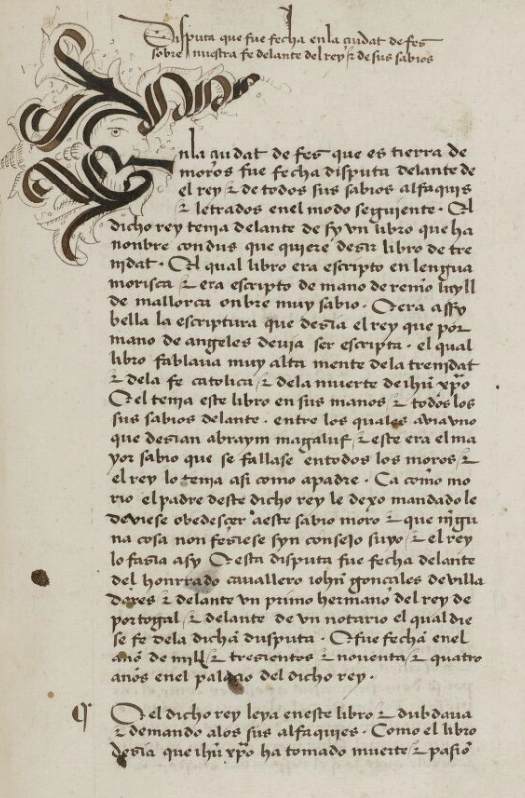
\includegraphics[width=0.5\textwidth]{HistoireIslamMediterranee/Images/DisputaFez1.png}
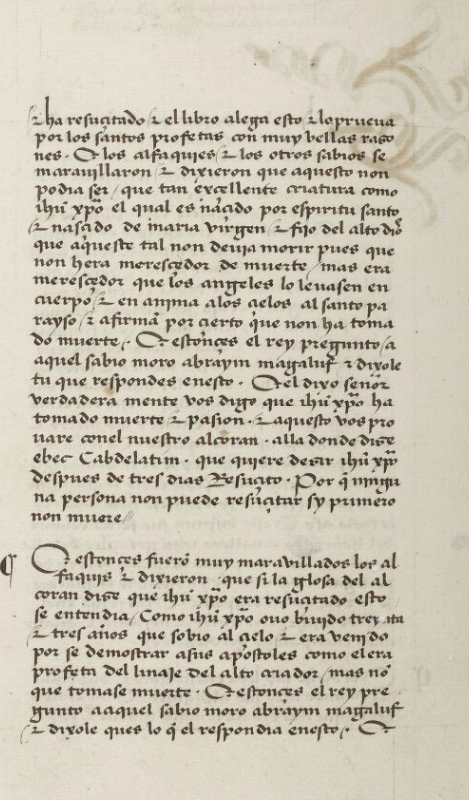
\includegraphics[width=0.5\textwidth]{HistoireIslamMediterranee/Images/DisputaFez2.png}
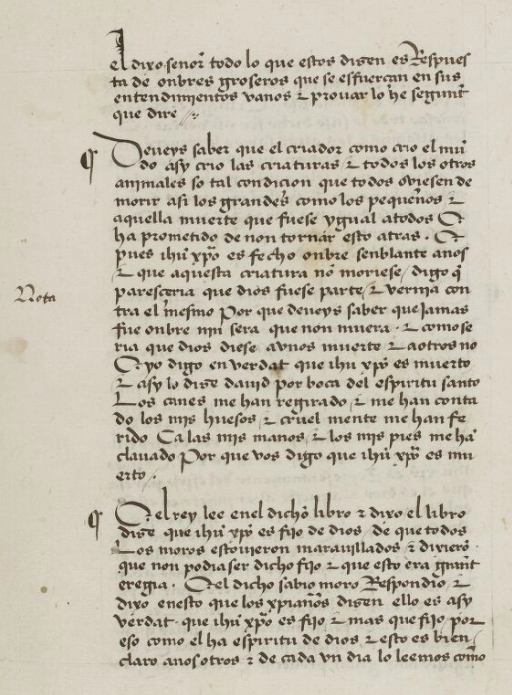
\includegraphics[width=0.5\textwidth]{HistoireIslamMediterranee/Images/DisputaFez3.png}
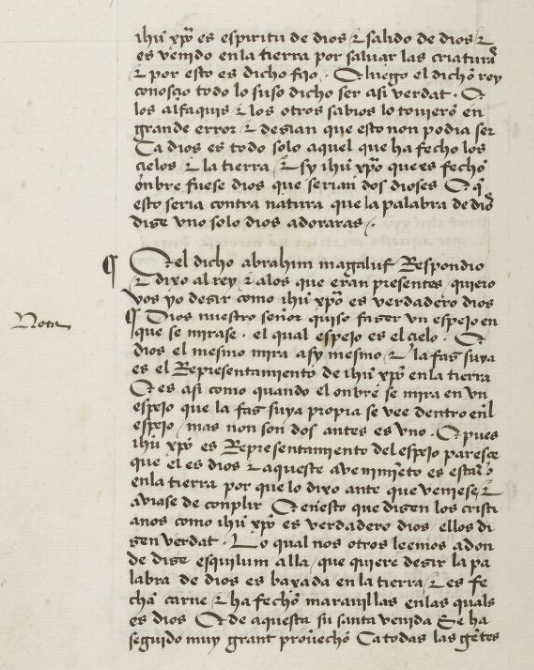
\includegraphics[width=0.5\textwidth]{HistoireIslamMediterranee/Images/DisputaFez4.png}
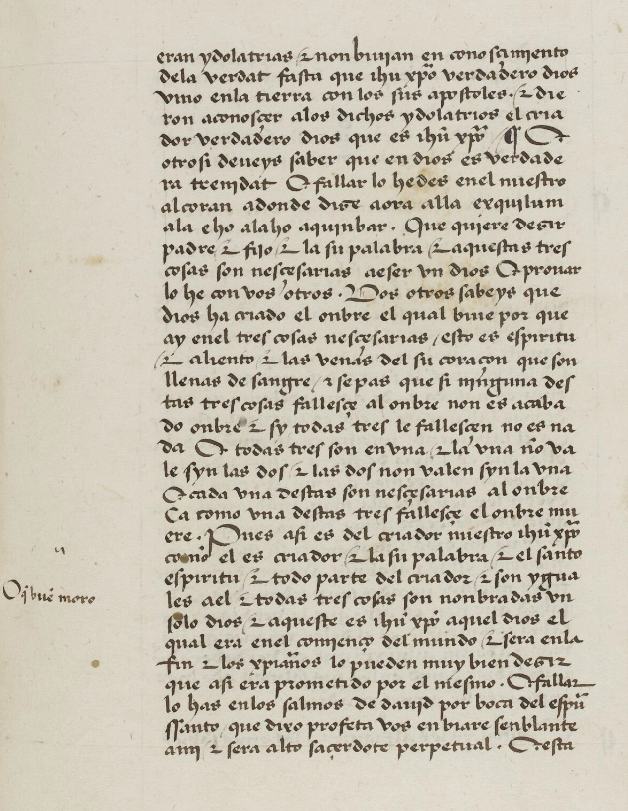
\includegraphics[width=0.5\textwidth]{HistoireIslamMediterranee/Images/DisputaFez5.png}
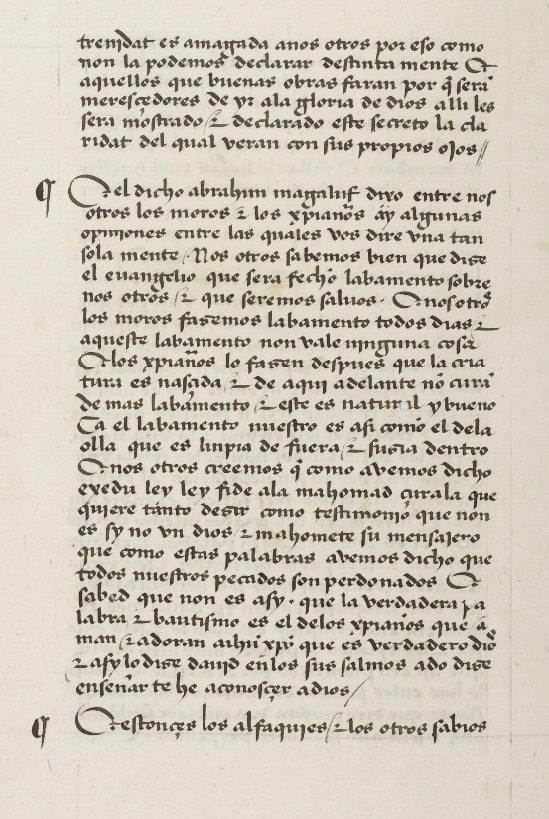
\includegraphics[width=0.5\textwidth]{HistoireIslamMediterranee/Images/DisputaFez6.png}
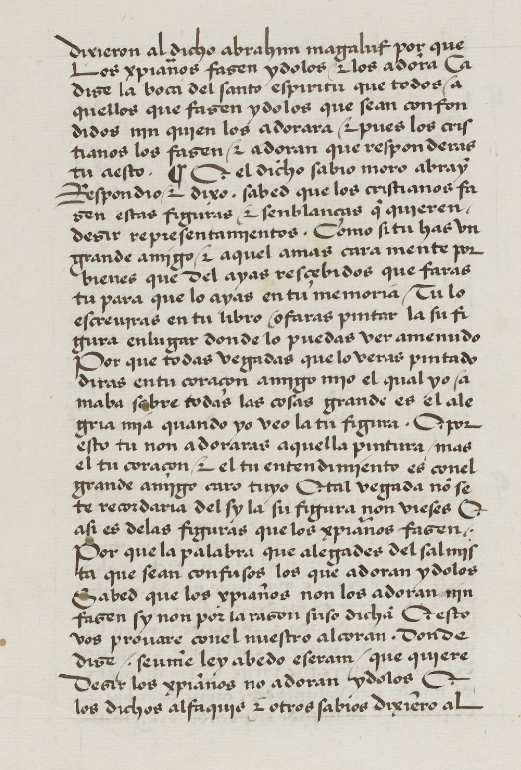
\includegraphics[width=0.5\textwidth]{HistoireIslamMediterranee/Images/DisputaFez7.png}
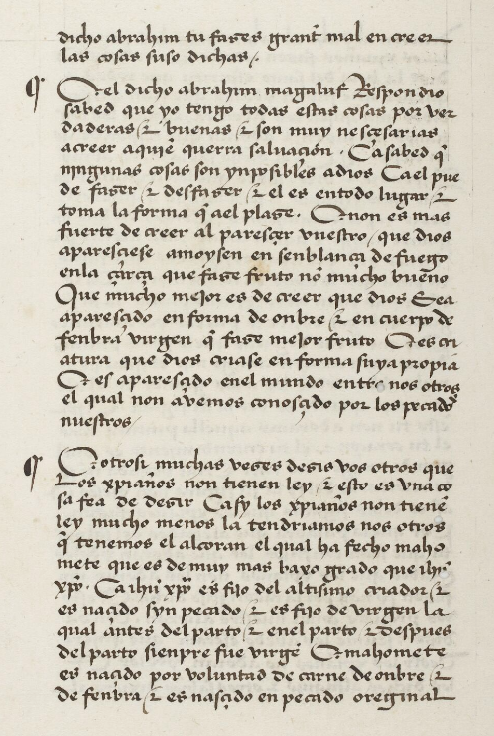
\includegraphics[width=0.5\textwidth]{HistoireIslamMediterranee/Images/DisputaFez8.png}
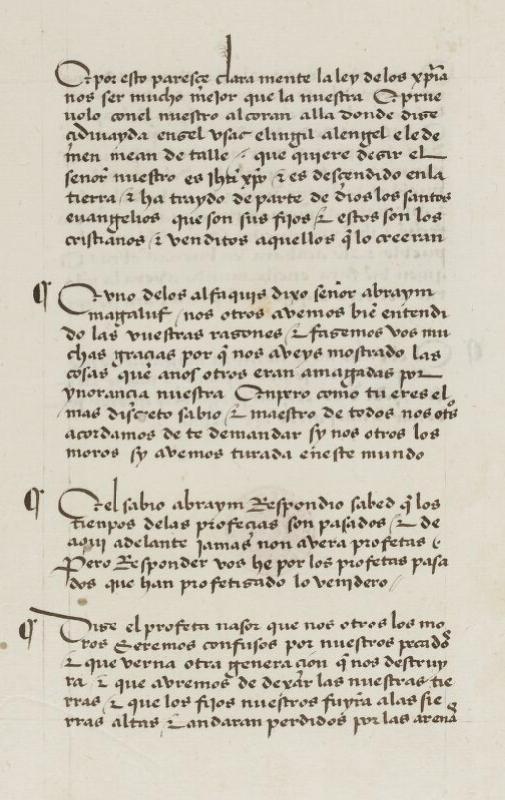
\includegraphics[width=0.5\textwidth]{HistoireIslamMediterranee/Images/DisputaFez9.png}
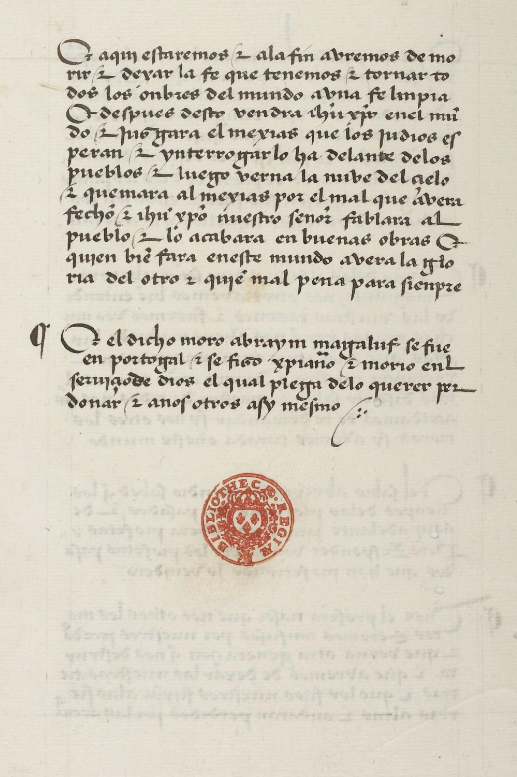
\includegraphics[width=0.5\textwidth]{HistoireIslamMediterranee/Images/DisputaFez10.png}
 
 
    \begin{longtable}{p{.48\textwidth}p{.48\textwidth}}
        Devete sapire che ne la dicta cità de Fes, d1'è in terra de'  r. 52.
Mori, fo facta disputatione denanci el Re e li suoi savi et ho  mini licterati sopra la fé nostra. E lo ditto Re se fe' portare in presencia sua un libro chiamato in lengua morescha <Conclus>,
5) che tanto significa corne <Libro de Trinità», il quale libro era scripto per mano de Raymundo Lull, naturale de l'île de Mayorica, Chrétien homo molto diligente. E parea tanto bella la scnptura che 'l Re dixe spesse volte essere scripta per mano de Dio; el quale libro profundamente tractava de Trinità e de la
10) sancta fé catholica et ancor de la morte de Jésus Christ. Et tenendolo el ditto Re nelle soe mano inseme con tucti suoi lic  terati, tra li guali havea un chiamato Abraym Magaluf, il.,,'quale era sopra tutti fontana di alta sciencia tenuto e reputato per lo Re corne a padre e pcr lo comune vuJgo per propheta. Per cio
15) che quando el Re vechio, padre del dicto Re, venne al morire, lasso et incarico al ditto suo fils , sotto pena de obediencia, che non facisse niuna cosa sença consiglyo de uesto savio moro.
E coss1 fe' e multo lo honoravano. Et ! la supra icta disputatione  1, 53 ,.
fo  fatta in conspetto del magnifico Johanne Gonçales de Villa
20) Dares e denanci a un fratello consobrino del Re de Portogallo e de un notaro il quale facesse fé de la ditta dispntatione, la quale fo facta nela ditta cità de Fes ne li milli ccc. xxxxiiii. nel palaço del ditto Re. E lo ditto Re, tenendo questo Libro de Trimtà ne le mano, legea in quello e, dubitando, domando alli
& Il faut savoir que dans la ville de Fes, en terre des morres, fo facta disputatione dénonce le Roi et ses sages et j'ai des mini litterati sur notre foi. Et ledit Roi fit porter devant lui un livre intitulé en langue mauresque <Conclus>,
5) ce qui signifie autant que <Livre de la Trinité», lequel livre a été écrit par la main de Raymundo Lull \sn{Raymon Lulle, Majorcain, Durant ses voyages, il écrivit de nombreuses œuvres pour démontrer ce qu'il considérait comme des erreurs des philosophes et des théologiens des autres religions. En partant de propositions communes aux trois religions du Livre, il montrait par combinaison que d'autres propositions étaient ou n'étaient pas compatibles avec ces premiers prédicats. Ses interlocuteurs qui acceptaient une proposition en apparence inoffensive étaient obligés de se rendre à ses conclusions. Il tenta également de fonder de nouveaux monastères catholiques dans les contrées qu'il visitait.}
, naturel de l'île de Mayorica, un homo Chrétien très diligent. Et l'écriture paraissait si belle que le Roi disait souvent qu'elle était écrite de la main de Dieu ; dans lequel livre traite en profondeur de la Trinité et de la
10) sancta fé catholica et ancora de la morte de Jésus Christ. Et ledit roi le tenant dans sa main avec tous ses licenciés, parmi eux il y avait un appelé Abraym Magaluf, le vuJgo per propheta. Ainsi
15) que lorsque le vieux Roi, père dudit Roi, vint à mourir, il partit et confia à son fils, sous peine d'obéissance, de ne rien faire sans l'avis de ce sage brun.
Et il fit ainsi, et ils l'honorèrent grandement. Et! le supra icta disputee 1, 53,.
réalisé en présence de la magnifique Johanne Gonçales de Villa
20) Donner et en espèces à un frère consobrine du roi du Portugal et à un notaire qui fait confiance à la société dispntatione, qui se fait en société de Fes dans le milli ccc. xxxxiii. dans le palais dudit Roi. Et ledit Roi, tenant ce Livre de Trimtà dans sa main, legea en lui et, doutant, demanda au
\\

25) soi savij alfaquini che am ditto libro dicea; gly quali nulla raione chiaramente sapeano dare. Et in quest'hora il ditto Re chiamo il ditto Abrahym Magaluf, il quale era maiore in sciencia de tutti quanti, e dixeli in substancia corne il libro dicea che Jésus Christ prese morte e passione per l'humana natura e che resu-
30) scito. E questo allegava il libro e provava per li sancti propheti con belle raxone. E Ji ditti savi che stavano in presencia del ditto Re forte se maraveglyaro e dixero che questo era impossi  bile e che tanto excellente creator corn'era Jésus Christ, nato per Spiritu Sancto dala Sacratissima Maria Vergene, havesse de
35) morire secondo che morte non meritava. Anci li convenia in corpo et in aria essere levato alli cieli ne] sancto paradiso, e affirmavano per certo quello non haver patuto morte. Li qual parole intesi per lo ditto Re, desiderando sapere la intencion del ditto Abrahym Magaluf, dixe: «Tu che dice in questo?» El quale
 & 
         
25) soi savij alfaquini qui m'a dit ce livre; gly que rien de la raison n'a clairement su donner. Et à cette heure le dit Roi appela le dit Abrahym Magaluf, qui était supérieur en science à tous, et dixeli en essence comme le livre dit que Jésus Christ prit la mort et la passion pour la nature humaine et qu'il ressuscita
30) Scythe. Et celui-ci a attaché le livre et a prouvé pour les sancti propheti avec un beau raxone. Et les dieux sages qui se tenaient en présence dudit roi fort s'émerveillèrent et dirent que cela était impossible et qu'un créateur aussi excellent que Jésus Christ, né par Spiritu Sancto de la Très Sainte Vierge Marie, avait de
35) mourir selon lequel la mort ne méritait pas. Même il leur convenait de corps et d'air d'être élevés au ciel dans le saint paradis, et ils affirmaient avec certitude qu'ils n'avaient pas subi la mort. J'ai entendu ces paroles par ledit Roi, désirant connaître l'intention dudit Abrahym Magaluf, il a dit: "Que dites-vous en cela?" El qui
         \\
    El quale
40) Abrahym, indriçando le sue parole al ditto Re chc lo havea in  terrogato, dixe: «Per certo ve dico che Jésus Christ prese morte e passione. E questo ve pruvo per lo mio Alchoram, dove dice
  
Ebe cabdelatim, che, retornandolo in vulgare, vol dire che Jésus Christ dopo de lre di resuscito. E manifcstamente appare che niuna persona po resuscitare se primo non more».  Et in  quel
puncto gly mori alfaquini stetero molto ammirati. Et respoxe un de loro dieendo per tutti: Che ancor che la I glosa de l'Alchoran dicesse che Jésus Christ resuscito, questo se intendea corn'ebbi
passati xxxiii. anni volse ascendere al ciclo c che non vinne per altro se non per demostrarse alli suoi apostoli com'era propheta de lo lignagio de l'alto creatore, ma non che patisse morte. Odendo el Re queste parole dixe al supraditto Abrahym: «Orche dice tu in questo»? Respoxe el ditto: \begin{quote}
    «Signor, quante cose questi dicano son resposte de persone grosse e pocho intelligentJ che se sforçano dire. Et intendol provar secondo oderiti»
\end{quote}. «Signor, dixe el ditto moro, quando el creator creo il mundo e l'homo e l'animali e tutte l'altre creature, fecili con tale conditione che tutti posissero morire, coss1 li grandi corne gly piccoli, e che co  mune a tutti fosse la morte, e. questo promise non tornar in  drieto. Adonque po' che Jésus Christ è fatto hom simile a noy e che non morisse, dicote che parerebi Idio essere parte e vene  rebi contra se stcsso. Et ancor più te dico chc may fo hom ne serà che non mora. E corne poterebbi essere che Idio donassi ad uni morte et ad altri no. E percio trovo in verità Jésus Christ essere morto, e questo confirma el propheta David per boccha del Spiritu Sancto: Li cani me hano ragirato et hanome contato gly mei ossa crudelmente, me hano ferito cbé le mie mano e gly mei pedi me banno chiavati. E per guesto ve dico che cer  tamente e morto».      & El qui
40) Abrahym, adressant ses paroles audit Roi qui l'avait interrogé, dit: «Je vous dis avec certitude que Jésus Christ a pris la mort et la passion. Et cela, je vous le prouve pour mon Alchoram, où il est dit
  
Ebe cabdelatim, qui, le ramenant au vernaculaire, signifie que Jésus Christ après de lre di resuscitato. Et il apparaît clairement que personne ne peut être ressuscité s'il ne meurt pas d'abord". Et en cela
puncto gly mori alfaquini était très admiré. Et respoxe l'un d'eux dieendo for all: Que même si le I glosa de l'Alchoran a dit que Jésus Christ resuscitato, cela si voulait dire corn'ebbi
passé xxxiii. ans, il voulut monter au cycle c qu'il ne gagna que pour se montrer à ses apôtres comme prophète de la lignée du haut créateur, mais non pour subir la mort. En entendant le Roi ces paroles, il dit au susmentionné Abrahym : « Où dis-tu là-dedans » ? Répondez à l'idem : \begin{quote}
    « Signor, combien de choses ces gens disent sont les réponses de gens grands et pas très intelligents qui s'efforcent de dire. Et j'ai l'intention d'essayer selon oderiti».
\end{quote} "Seigneur, dit le ténébreux idem, quand le créateur a créé le monde et l'homme et les animaux et toutes les autres créatures, je les ai faits dans une telle condition que tout le monde pouvait mourir, donc les grandes cornes étaient petites, et ce qui est commun à tous était la mort, e. ce qu'il a promis de ne pas revenir. Donc, tandis que Jésus Christs a été fait comme nous et n'est pas mort, vous dites qu'il semble à Dieu d'être une partie et d'être retenu contre lui-même. Et même plus je vous dis qu'il se peut que pour lui il ne meure pas. Et comment se pourrait-il que Dieu ait accordé la mort à certains et non à d'autres. Et donc je trouve en vérité que Jésus Christ est mort, et cela est confirmé par le prophète David par la bouche du Saint-Esprit : Les chiens m'ont volé et ont cruellement compté mon nom avec mes os, ils m'ont blessé avec mes mains et mes pieds ils m'ont battu. Et pour cela, je vous dis qu'il est certainement mort. \\
E tutti l'altri mon concederono e con  cordarono col ditto sagio moro. Dopo el Re legendo el Re nel ditto libro dicea che Jésus Christ era fils de Dio. De la qual cosa tutti li mori furon amirati et dixeno al Re che non era possibile che sia ditto fils perché parerebi grande heresia. E lo ditto savio moro Ahrahym resposc: «In quello che li xpistiani diceno, lor diceno hona ragione e vera clie Jésus Christ
era fils de Dio e più che figlyo, per cio che I lui tene spiritu
de D10. E questo a noy è ben chiaro, et ogni dà lo legemo, corne Jésus Christ è spiritu de Dio et è enscito da Dio et in terra è dexciso per salvare la natura humana. E per questo è ditto fils ». Et mcontenente el ditto Re conob1 questo essere in verità per le propationi sopradicte.
Eli alfaquini e tutti l'altri savi mori ténerlo in grande errore dicendo clie questo no possiva essere perché ldio era tutto solo colui che fe  i cieli e la terra. Et si Jésus Christ chi è fatto
85) homo fosse Dio, serebino doi Dei. E questo serebi contro natura, ché la parola de Dio dice: Un solo Dio adoreray. E lo ditto Abrahym Magaluf respoxe e dîxe: 

& 

Et tous les autres Mons ont concédé et convenu avec ledit sage Maure. D'après la légende, le Roi dit dans ledit livre que Jésus Christ était un fils de Dieu dont tous les morts étaient admirés et dit au Roi qu'il n'était pas possible qu'il soit appelé un fils car ils semblaient être un grand hérésie. Et ledit sage Moor Ahrahym répondit: «Dans ce que disent les xpi stani, ils disent juste et vrai que Jésus Christ
il était un fils de Dieu et plus qu'un figlyo, pour ce que je lui tene spiritu
de D10. Et cela est très clair pour nous, et tout le monde donne le legem, car Jésus Christ est l'esprit de Dieu et est venu de Dieu et a été décidé sur terre pour sauver la nature humaine. Et pour cette raison, on l'appelle fils ». Et l'homme contenant ledit Roi savait cet être en vérité par les propositions ci-dessus.
Eli Alfaquini et tous les autres sages l'ont gardé dans une grande erreur en disant que cela ne pouvait pas être parce que Dieu était tout seul qui a fait les cieux et la terre. Et si Jésus Christ qui est fait
85) homo était Dieu, serebino doi Dei. Et cela était contre nature, car la parole de Dieu dit : Vous n'adorerez qu'un seul Dieu. Et le idem Abrahym Magaluf respoxe e dîxe : \\

«Gly xpistiani diceno che Jésus Christ è vero Dio e dicono verità. El quale noy legemo dove
&

« Les Gly xpistiani disent que Jésus Christ est le vrai Dieu et ils disent la vérité. El que nous lisons où \\
dice: Esquilitimus alla; chc vol dire: la parnla de .Dio è discesa
90) in nela terra et è fatta carne et ha fatte maraviglyose cose, in ne]i quali è Dio. Et devete sapire cbe ldio è ,·cta Trinità; e qucsto troveray ne] nostro Alchoran dovc <lice: Aora alla cxquilim ala co alaho aquibar; che,·o'  dire: Padre c figlyo e la sua parola. E 'lueste tre cose son necessaric ad esserc un Dio. E questo pro-
95) viro con vui altri. Voi doveti sapire che Tclio ha creato l'homo, i] quale vive in qucsto mundo, che in quello son trc cose nc  cessarie: cio è spirituali e fiato e le,·ene del rore che son pieni de sangue; et è manifesto chc s'alcuna de queste trc cose manca è niente, e se tutti tre cose mancano tanto pegio, e tut.te t:re
100) son necessaric, e l 'una sença li doi no valc c manco Ji doi sença l'una. E ciascuna de queste son neces:;arie a l'homo. E quando l'una de queste manea l'homo more. Adonque eoss, è de] crea  tore nost:ro Jésus Christ corne lui è creatorc c la sua parola è lo Spiritu Sancto e t-utto procedc daJ crcatore c sono equali a Hui.
105) c tutti tre son chiamati  un solo Dio,  chi  cra  in  ne] 1 principio  1. s .
delmundo e serà in ne La fine. E quello che li xpistiani dicono è multo verità grande, ché coss1 era promesso per Dio, la qua! cosa troveray ncgly psalmi de David per bocca del Spiritu Sancto, quai dixe: «Propheta vc mandero simile a me e serà alto sacer-
110) dote pcrpetuale. E. devete sapire cbc le dittc cose significano Trinità, con tutto che sia a noy secreta. Pertanto corne sia di  stinctamente non se puù per noy dcclara.rc. E quelli che ben adoprano anderanno alla gloria de Dio, dove serà dcclarato e mostrato questo secreto; el quaJc secret·o Yederanno apertamentc
115) con li suoi proprij ochi». &

dit : Esquilitimus alla ; ce qui signifie : la parole de Dieu est descendue
90) sur la terre, il s'est fait chair et a fait des choses merveilleuses, dans lesquelles Dieu est.Et vous devez savoir ce qu'est Dieu, la Trinité; et ceci vous trouverez dans] notre Alchoran où <lice: Aora alla cxquilim ala co alaho aquibar; cela,·ou' dire : Père c figlyo et sa parole. Et ces trois choses sont nécessaires pour qu'il y ait un Dieu.
95) Je vis avec vous autres. Vous devez savoir qu'il a créé l'homme, qui vit dans ce monde, que dans ce monde il y a trois choses qui ne sont pas nécessaires : c'est-à-dire les esprits et le souffle et les flammes qui sont pleines de sang ; et il est clair que s'il manque l'une de ces trois choses, ce n'est rien, et s'il manque les trois choses, c'est encore pire, et tout
100) ils sont nécessaires, et le una sença li doi no valc c manque Ji doi sença l'una. Et chacun d'eux est nécessaire : des airs à l'homo. Et quand l'un d'eux affecte davantage l'homo. Par conséquent, il est de] notre créateur Jésus Christ car il est créateur c sa parole est le Spiritu Sancto et tous les procédés du créateur c sont égaux à Hui.
105) c tous les trois sont appelés un seul Dieu, qui cra in ne] 1 principe 1. s .
delmundo et sera dans ne La fin. Et ce que disent les xpistiani est une très grande vérité, car cela a été promis par Dieu, ici ! que trouverez-vous ncgly psaumes de David par la bouche du Spiritu Sancto, quai dixe: «Propheta vc j'enverrai semblable à moi et il sera grand prêtre-
110) dot perpétuelle. E. vous devez savoir comment les choses dictées signifient la Trinité, avec tout ce qu'elle nous est secrète. Donc comme d'instinct c'est pas possible pour nous dcclara.rc. Et ceux qui font bien iront à la gloire de Dieu, où ce secret sera déclaré et révélé ; el quaJc secret · ou ils donneront ouvertement
115) de ses propres yeux». \\

Et ancor pit1 il di tto Abrahym Magaluf dixe al Re et a quelli chi presenti erano: «Io ve voglyo mostrare el vero Dio nel mundo. Dio nostro signore volse fare un spechio, cio è nel cielo in ne] qualc mira sé stesso, e la faça sua è re  presentatione de Yhcst1 Christ in  nc]a terra; è proprio cuss1 como
120) qui ]'omo se mira in uno spechio e rnde m dcntro sua propria
similitudine, ma gi11 pcr qucsto 11011 sono doi, ma 11110. E po' che  Jésus  Christ è representationc del spcchio pare eb·è Dio. E questo aveuimento è stato a la terra pcrchè  nante che vcnissc
]o dixe et era necessario se haYcsse de scquire. e de quesla sua
125) sancta venuta se ne ha scquito grande utilill1; tuui Ji gcnti erano ydolatri e non veniano in co11oscimento de la verità finché Jésus Christ venne in ne la terra, il quale con gly,moi apostoli det  tero a conoscere a li ditti ydolatri cl crcatore vostro Dio essere Jésus Christ)).
&
Et encore plus le dito Abrahym Magaluf dit au Roi et à ceux qui étaient présents : « Je veux te montrer le vrai Dieu dans le monde. Dieu notre seigneur a voulu faire un miroir, c'est-à-dire qu'il est dans le ciel en quelque point de lui-même, et son visage est la représentation de Yhcst1 Christ dans n]a terre ; c'est juste cuss1 como
120) ici l'homme se regarde dans un miroir et se voit dans son propre
similitude, ma gi11 pcr qucsto 11011 sono doi, ma 11110. C'est juste que Jésus Christ est la représentationc du miroir semble-t-il et il est Dieu. Et cet événement était sur terre parce que nante que vcnissc
]o dixe et était nécessaire si haYcsse de scquire. et de celui-ci son
125) sainte venue, il en a fait grand usage1; tous les Juifs étaient des idolâtres et ne sont pas parvenus à la connaissance de la vérité jusqu'à ce que Hest1 Christ soit venu sur la terre, qui avec gly, nos apôtres ont fait connaître aux idolâtres que le chercheur de votre Dieu était Yhesu Christ)). \\
    \end{longtable}
 